\let\negmedspace\undefined
\let\negthickspace\undefined
\documentclass[journal,12pt,twocolumn]{IEEEtran}
\usepackage{gensymb}
\usepackage{amssymb}
\usepackage[cmex10]{amsmath}
\usepackage{amsthm}
\usepackage{amsmath}
\usepackage{enumitem}
\usepackage{mathtools}
\usepackage{listings}
\usepackage{color}                                            %%
\usepackage{hhline}                                           %%
\usepackage{ifthen}                                           %%
\usepackage{lscape}    
\usepackage{graphicx}
\title{\textbf{Assignment-1}}
\author{Chittepu Rutheesh Reddy \\
  cs21btech11014}
  \begin{document}
\maketitle{}

\subsection*{\textbf{4b[ICSE 2018]}}
If the straight lines $3x- 5y = 7$ and $4x+ ay+ 9 = 0$ are perpendicular to one 
another, find the value of a.

\subsection*{\textbf{Solution}}
If two lines are perpendicular, then dot product of their direction ratios is 0.
\bigskip

 Vector form of 3x - 5y =7 is \textbf{r1} = $\binom{4}{1} + t1\binom{5}{3}$,\, with $\binom{5}{3}$ as direction ratio.
 \bigskip
   
 Vector form of 4x+ay+9=0 is \textbf{r2} = $\binom{\frac{-9}{4}}{0} + t2\binom{a}{-4}$,\, with $\binom{a}{-4}$ as direction ratio.
  \\
   
   As  \,\,  $\binom{5}{3}$.$\binom{a}{-4}$= 0
   \\ 
   
    5a - 12 = 0 
  \\
 
   So  \,  $a = (\frac{12}{5})$ \\
   \\\\\\\\\\\\\\\\\\\\\\\\\\
  
  \graphicspath{{D:/Semester 2/Probability and Random Variables AI1110/Assignments/1/}}   
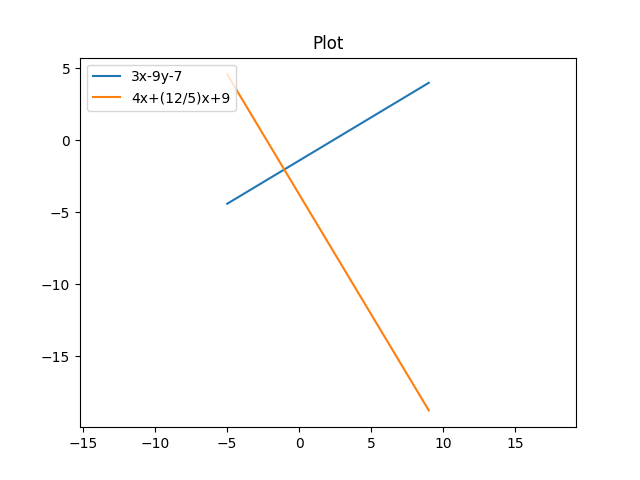
\includegraphics[scale=0.6]{Figure_1}

\end{document}